% %%%%%%%%%%%%%%%%%%%%%%%%%%%%%%%%%%%%%%%%%%%%%%%%%%%%%%%%%%%%
\section*{Materials and Methods}
% %%%%%%%%%%%%%%%%%%%%%%%%%%%%%%%%%%%%%%%%%%%%%%%%%%%%%%%%%%%%

% ------------------------------------------------------------
\subsection*{Animals}
% ------------------------------------------------------------

We conducted all experiments in adult transgenic mice (8--20 weeks)
expressing either GCaMP6s or GCaMP8s in excitatory cortical neurons
under the CaMKII promoter. To enable simultaneous wide-field calcium
imaging and optogenetic perturbation, animals received a retro-orbital
injection of a PHP-eB serotype adeno-associated viral (AAV) vector
carrying a DLX2.0-driven Chrimson construct, which restricts opsin
expression to inhibitory interneurons and thereby enables focal cortical
suppression through inhibitory activation with minimal spectral
cross-talk with GCaMP imaging. This dual-expression configuration
permitted mesoscale calcium measurement via GCaMP fluorescence and
spatially localized, optogenetically driven suppression within the same
field of view. All procedures were approved by the Institutional Animal
Care and Use Committee (IACUC) at the University of Washington and were
conducted in accordance with NIH guidelines for the care and use of
laboratory animals.

% ------------------------------------------------------------
\subsection*{Surgical preparation and habituation}
% ------------------------------------------------------------

We implanted a chronic trans-cranial window over the dorsal cortex to
provide stable, long-term optical access to the entire dorsal cortical
surface in awake animals, following procedures described previously
\citep{Matveev2024}. Briefly, we removed the scalp and periosteum and
applied thin layers of UV-cured optical glue to the exposed skull
surface inside a 3D-printed recording chamber secured with dental
cement, maintaining transparency over the imaging field of view. We
attached a custom head-plate to allow reproducible head-fixation across
sessions. Animals were allowed at least one week of recovery before any
experimental handling.

% ------------------------------------------------------------
\subsection*{Wide-field calcium imaging}
% ------------------------------------------------------------

We recorded neural activity using a custom single-photon mesoscopic
fluorescence microscope with excitation and emission filters matched to
the GCaMP spectrum. We acquired images at 70\,Hz with a
$9.7\,\mathrm{mm} \times 9.7\,\mathrm{mm}$ field of view, providing
mesoscale coverage of the entire dorsal cortical surface at a pixel
resolution sufficient to resolve regional population dynamics. We
collected frames using alternating blue (470\,nm) and violet (405\,nm)
illumination at 35\,Hz per channel; the violet channel captures
hemodynamic absorbance and tissue autofluorescence for correction
purposes and was not used for real-time computation. We maintained light
power below levels known to elicit phototoxicity or direct
photostimulation of Chrimson.

For offline analysis, we preprocessed imaging data using a standard
pipeline including rigid motion correction, reflectance normalization,
and computation of $\Delta F/F$. We registered frames to a common
anatomical reference atlas and temporally aligned stimulation event
timestamps to the imaging data stream for trial-level analysis. Full
hardware specifications, surgical details, and viral constructs are
described in \citet{Matveev2024}.

% ------------------------------------------------------------
\subsection*{Optogenetic stimulation}
% ------------------------------------------------------------

We delivered optogenetic stimulation concurrently with imaging via a
secondary, spatially targeted illumination pathway tuned to the Chrimson
activation spectrum (638\,nm). A galvanometer-steered laser beam
confined stimulation to a user-defined cortical region, specified as a
two-dimensional coordinate relative to Bregma in the control software.
The stimulation target was positioned in a cortical region neighboring
the $\Delta F/F$ output zone, chosen such that the spatial spread of
optogenetic activation encompassed the output region. We calibrated
light power before each session using a power meter positioned at the
objective focal plane. We delivered stimulation pulse trains or
constant-power steps as analog voltage commands from a microcontroller,
with a linear mapping between command voltage (0--5\,V) and light power
(0--36\,mW). We capped peak light power at 36\,mW to remain within the
unsaturated, physiologically safe operating range of the opsin. We
verified spectral separation between the GCaMP excitation band and the
Chrimson activation band before each cohort of experiments; no
measurable cross-talk was observed.

% ------------------------------------------------------------
\subsection*{Real-time closed-loop system}
% ------------------------------------------------------------

\subsubsection*{Hardware and software architecture}

We implemented the real-time experimental system in Python on a
dedicated control server (CS). We acquired wide-field images using the
Pylon image-capture API and streamed them directly to the CS at 70\,Hz.
Only blue-channel frames (35\,Hz effective rate) were used for real-time
computation; we discarded violet frames during online processing. The CS
displayed real-time images, $\Delta F/F$ traces, and experimental
parameters via a graphical user interface (GUI). A dedicated computation
thread processed incoming frames, computed the feedback signal,
evaluated the controller, and transmitted stimulation commands to a
microcontroller unit (MCU). The MCU performed digital-to-analog
conversion and drove the optogenetic stimulation hardware. A separate
logging thread recorded all event timestamps---including image
acquisition triggers, controller outputs, and stimulation
commands---to disk for offline analysis.

The complete control loop, from camera exposure trigger to stimulation
command delivery, had a measured end-to-end latency of approximately
80\,ms (Fig.~\ref{fig:figure1}F), arising from image transfer (${\sim}15$\,ms),
$\Delta F/F$ computation (${\sim}30$\,ms), and digital-to-analog
conversion and stimulator settling (${\sim}35$\,ms).

\subsubsection*{Online signal processing}

We computed the real-time feedback signal as the mean $\Delta F/F$
within a circular kernel centered on the designated output region in
somatosensory cortex. The $\Delta F/F$ signal was defined as
%
\begin{equation}
    y_{t} = \frac{F_{t} - \bar{F}}{|\bar{F}|},
    \label{eq:dff}
\end{equation}
%
where $F_{t}$ is the kernel-averaged fluorescence at frame $t$ and
$\bar{F}$ is the running-window mean computed over a preceding baseline
window of fixed duration. The sign convention in the denominator ensures
that $y_{t}$ correctly represents fractional change even when $\bar{F}$
is negative, which can occur due to hemodynamic artifacts in uncorrected
signals. We computed and visualized the $\Delta F/F$ trace continuously
on the GUI throughout the session.

\subsubsection*{Trial structure and experimental design}

We delivered optogenetic stimulation in discrete trials of 3\,s
duration, separated by 15\,s inter-trial intervals (ITIs) during which
no stimulation was applied and the animal rested. We set the reference
signal to $y_{\mathrm{ref}} = -5\%\,\Delta F/F$ for the entire 3\,s
stimulation window, corresponding to a target suppression of 5
percentage points relative to the running baseline. Each session
comprised 100 validation trials, of which half were randomly designated
as closed-loop trials (feedback active) and half as open-loop trials
(feedforward only), interleaved in a pseudorandom order. This
interleaving ensured that the two conditions sampled the same
distribution of brain states within each session. Each session began
with a controller tuning phase (see Section~\ref{sec:gain_opt}), after
which the 100-trial validation block was initiated. Total experiment
duration was approximately 1\,h per session.

% ------------------------------------------------------------
\subsection*{Mathematical framework}
% ------------------------------------------------------------

\subsubsection*{Nonlinear system model}

We modeled the cortical response dynamics at the output region as a
nonlinear, parameter-varying system driven by optogenetic input:
%
\begin{align}
    x_{t+1} &= f(x_{t},\,u_{t},\,\rho_{t}) + d_{t} + w_{t},
               \label{eq:nl_state} \\
    y_{t}   &= h(x_{t},\,u_{t},\,\rho_{t}) + v_{t},
               \label{eq:nl_out}
\end{align}
%
where $x_{t} \in \mathbb{R}^{n}$ is the low-dimensional latent cortical
state, $u_{t} \in \mathbb{R}$ is the scalar optogenetic input,
$\rho_{t} \in \mathbb{R}^{p}$ is a time-varying parameter vector
encoding spontaneous brain-state fluctuations (e.g., arousal, movement,
cortical synchrony), $d_{t} \in \mathbb{R}^{n}$ is an internal
disturbance representing unobserved inputs from other brain regions,
$w_{t} \in \mathbb{R}^{n}$ is bounded process noise, $y_{t} \in
\mathbb{R}$ is the measured $\Delta F/F$ output, and $v_{t} \in
\mathbb{R}$ is measurement noise. The functions $f$ and $h$ are assumed
continuous but otherwise unknown. The wide-field $\Delta F/F$ activity
is biologically bounded, implying that the system
\eqref{eq:nl_state}--\eqref{eq:nl_out} is marginally stable with
oscillatory dynamics near a stationary mean. We write the state
transition as
%
\begin{equation*}
    x(t) = \Phi(x_{0},\,u,\,d,\,\rho), \qquad
    y(t) = h \circ \Phi(x_{0},\,u,\,d,\,\rho),
\end{equation*}
%
where $\Phi$ is the transition map. We assume that the initial condition
$x_{0}$ is drawn from the stationary distribution of the system,
$x_{0} \sim \mathcal{D}$, with $\mathbb{E}[x_{0}] = \bar{x}_{0}$, and
that the disturbances $d$ and brain states $\rho$ are sampled from
stationary distributions. Applying an input sequence $u_{0}, \ldots,
u_{t-1}$ yields a sample of the output trajectory $Y_{0:T}$.

\subsubsection*{Linear parameter-varying approximation}

Because $f$ and $h$ are unknown and $\rho_{t}$ cannot be measured
directly, exact nonlinear control is infeasible. We instead adopt a
linear parameter-varying (LPV) approximation that captures the dominant
input--output structure:
%
\begin{align}
    x_{t+1} &= A(\rho)\,x_{t} + B(\rho)\,u_{t} + w_{t} + d_{t},
               \label{eq:lpv_state} \\
    y_{t}   &= C\,x_{t} + v_{t},
               \label{eq:lpv_out}
\end{align}
%
where
\begin{equation*}
    A(\rho) = \sum_{k=1}^{n} \rho_{k} A_{k}, \qquad
    B(\rho) = \sum_{k=1}^{n} \rho_{k} B_{k},
\end{equation*}
and the parameter $\rho$ varies across trials due to spontaneous
fluctuations in arousal, behavioral state, and network dynamics. We
assume the disturbances $d_{t}$ and noise terms $w_{t}$, $v_{t}$ are
bounded and zero-mean. Because the distribution of $\rho$ cannot be
estimated reliably within experimental constraints, conventional system
identification (frequency sweeps, persistent excitation, subspace
methods) is infeasible. Physiological constraints also limit the
amplitude and duration of permissible inputs, the number of trials per
session, and total recording time. We therefore adopt a model-free
approach to controller design grounded in Assumption~\ref{assm:trial_avg}
below.

\subsubsection*{Trial-averaging assumption}

Let $Y_{0:T} = y_{0}, y_{1}, \ldots, y_{T}$ denote the output
trajectory generated by the nonlinear system
\eqref{eq:nl_state}--\eqref{eq:nl_out} under input sequence
$U_{0:T-1} = u_{0}, \ldots, u_{t-1}$, with initial condition $x_{0}
\sim \mathcal{D}$ and disturbances and brain states drawn from
distributions $\mathcal{P}$ and $\mathcal{Q}$, respectively. We
hypothesize that the trial-averaged nonlinear dynamics are well
described by a linear time-invariant (LTI) system that requires no
knowledge of brain states or disturbances. Consider the nominal LTI
system
%
\begin{align}
    x_{t+1} &= \bar{A}\,x_{t} + \bar{B}\,u_{t}, \label{eq:lti_state}\\
    y_{t}   &= C\,x_{t},                          \label{eq:lti_out}
\end{align}
%
whose output trajectory is $\bar{Y}_{0:T} = \mathcal{A}\,x_{0} +
\Gamma\,U_{0:T-1}$, where $\mathcal{A}$ and $\Gamma$ are constructed
from $\bar{A}$, $\bar{B}$, and $C$.

\begin{assumption}[Trial-averaging]
\label{assm:trial_avg}
The trial-averaged output sequence of the nonlinear system
\eqref{eq:nl_state}--\eqref{eq:nl_out} is well approximated by the
output sequence of the nominal LTI system
\eqref{eq:lti_state}--\eqref{eq:lti_out} with zero disturbance and
zero-mean noise:
\begin{equation}
    \mathbb{E}\!\left[Y_{0:T}(x_{0},\,u,\,d,\,\rho)\right]
    = \bar{Y}_{0:T}(x_{0},\,u),
    \label{eq:trial_avg}
\end{equation}
where $Y_{0:T}$ denotes the output trajectory of the nonlinear system
initiated at $x_{0}$, and $\bar{Y}_{0:T}$ denotes the output trajectory
of the nominal LTI system initiated at $\bar{x}_{0} =
\mathbb{E}[x_{0}]$. The parameter $\rho \in \mathcal{P}$ and
disturbances $d \in \mathcal{Q}$ are drawn from bounded, stationary
sets such that $\mathbb{E}[d_{t}] = 0$ and $\mathbb{E}[\rho_{t}] =
\bar{\rho}$ hold approximately over the session.
\end{assumption}

Under Assumption~\ref{assm:trial_avg}, trial-to-trial deviations from
the averaged response are due to zero-mean perturbations that cancel in
expectation. The nominal system $(\bar{A},\bar{B},C)$ therefore provides
the effective input--output model on which the controller is designed.
We provide empirical support for this assumption by analyzing the
variance of trial responses across batch sizes (Fig.~\ref{fig:S1}).

% ------------------------------------------------------------
\subsection*{System characterization}
% ------------------------------------------------------------

\subsubsection*{Impulse response protocol}

To assess the linearity and monotonicity of the input--output
relationship, we delivered impulse-like optogenetic inputs at varying
amplitudes sampled from a discrete set (0, 0.8, 1.6, 2.4, 2.7\,V),
interleaved with randomized inter-trial intervals and delivered in
pseudo-random amplitude order. We quantified the response to each
amplitude level as the mean peak \%\,$\Delta F/F$ suppression across
trials, where we determined peak timing from the trial-averaged waveform
at the highest stimulus amplitude. We used a linear regression of peak
suppression on stimulus amplitude to assess input--output linearity and
to estimate the feedforward gain $K_{r}$ (see
Section~\ref{sec:ff_gain}). We required a minimum of 20 trials per
amplitude level for inclusion in the linear fit.

\subsubsection*{Step response protocol}

To characterize steady-state dynamics and estimate the effective gain of
a sustained stimulus, we applied a constant optogenetic input at a fixed
voltage for 3\,s trial windows, with trials spaced by a fixed ITI
across the session. We compared the trial-averaged step response to its
within-window mean as a proxy for steady-state output. We also computed
variance across trials as a function of time to assess the stability of
the response and the validity of Assumption~\ref{assm:trial_avg} across
sessions.

% ------------------------------------------------------------
\subsection*{Controller design}
% ------------------------------------------------------------

\subsubsection*{Feedforward gain calibration}
\label{sec:ff_gain}

The feedforward component of the controller provides the nominal input
required to achieve an output close to $y_{\mathrm{ref}}$, compensating
for the baseline gain of the optogenetic actuator. The feedforward
command at each timestep is:
%
\begin{equation}
    \bar{u}_{t} = K_{r}(y_{\mathrm{ref}} - y_{t}),
    \label{eq:ff}
\end{equation}
%
where $K_{r}$ is a scalar gain estimated from the impulse response
calibration experiment. Let $U = [u_{1}, \ldots, u_{K}] \in
\mathbb{R}^{1 \times K}$ be the row vector of stimulus amplitudes and
$Y = [(y_{1} - y_{\mathrm{ref}}), \ldots, (y_{K} - y_{\mathrm{ref}})]
\in \mathbb{R}^{1 \times K}$ the corresponding trial-averaged output
deviations from the reference. The least-squares feedforward gain is:
%
\begin{equation}
    K_{r} = U Y^{\dagger},
    \label{eq:kr}
\end{equation}
%
where $Y^{\dagger}$ denotes the Moore--Penrose pseudoinverse. This
estimate provides an approximate open-loop inversion of the
input--output map and serves as the baseline for PI feedback
augmentation.

\subsubsection*{Proportional--integral feedback controller}
\label{sec:pi_controller_design}

To compensate for model bias in $K_{r}$, residual nonlinearities,
trial-to-trial disturbances, and brain-state-dependent deviations that
the feedforward term cannot correct, we appended a
proportional--integral (PI) feedback controller to the feedforward
command. The total stimulation input at each timestep is:
%
\begin{equation}
    u_{t} = K_{r}(y_{\mathrm{ref}} - y_{t})
          + K_{p}(y_{\mathrm{ref}} - y_{t})
          + K_{i}\sum_{k=0}^{t}(y_{\mathrm{ref}} - y_{k})\,\Delta t,
    \label{eq:pi}
\end{equation}
%
where $K_{p} > 0$ is the proportional gain and $K_{i} > 0$ is the
integral gain. The proportional term provides timestep-level correction
proportional to the instantaneous tracking error; the integral term
accumulates signed error across the trial to eliminate persistent bias.
We applied anti-windup clamping to the integral accumulator to prevent
integrator saturation during periods when the actuator is saturated. We
clipped the command $u_{t}$ to the feasible range $[0, 5\,\mathrm{V}]$
before transmission to the optogenetic stimulator, corresponding to a
maximum light power of 36\,mW.

In the open-loop condition, we set feedback gains to $K_{p} = K_{i} =
0$, reducing \eqref{eq:pi} to the feedforward term \eqref{eq:ff} alone.
This provides the comparison baseline against which we evaluate
closed-loop performance.

\subsubsection*{Augmented state representation}

To facilitate analysis of the closed-loop system under
Assumption~\ref{assm:trial_avg}, we represent the integral action in
\eqref{eq:pi} as an augmented state variable $\xi_{t} = \sum_{k=0}^{t}
(x_{k} - x_{\mathrm{ref}})\,\Delta t$. The augmented state vector
$s_{t} = [x_{t}^{\top},\,\xi_{t}^{\top}]^{\top}$ satisfies:
%
\begin{align}
    \begin{bmatrix} x_{t+1} \\ \xi_{t+1} \end{bmatrix}
    &= \begin{bmatrix} \bar{A} & 0 \\ I\,\Delta t & I \end{bmatrix}
       \begin{bmatrix} x_{t} \\ \xi_{t} \end{bmatrix}
    +  \begin{bmatrix} \bar{B} \\ 0 \end{bmatrix} u_{t},
    \label{eq:aug_state} \\
    y_{t} &= \begin{bmatrix} C & 0 \end{bmatrix} s_{t}.
    \label{eq:aug_out}
\end{align}
%
The feedback control law takes the compact form $u_{t} = K s_{t}$,
where $K = [K_{p},\,K_{i}]$. Under Assumption~\ref{assm:trial_avg}, the
closed-loop system \eqref{eq:aug_state}--\eqref{eq:aug_out} with $u_{t}
= K s_{t}$ is stable provided $K_{p}$ is consistent with the
approximately monotonic input--output relationship established
empirically \citep{Astrom1995}.

% ------------------------------------------------------------
\subsection*{Controller gain optimization}
\label{sec:gain_opt}
% ------------------------------------------------------------

\subsubsection*{Performance metric}

We quantified controller performance using the mean-squared tracking
error accumulated over each trial. The per-trial tracking cost for an
experiment initiated at latent state $x_{0}$ under gain $K$ is:
%
\begin{equation}
    c(x_{0};\,K) = \sum_{t=0}^{T} \|z(t)\|^{2},
    \qquad z(t) = y_{t} - y_{\mathrm{ref}},
    \label{eq:trial_cost}
\end{equation}
%
and the expected cost over the distribution $\mathcal{D}$ of initial
conditions and brain states is:
%
\begin{equation}
    J(K) = \mathbb{E}_{x_{0} \sim \mathcal{D}}\!
           \left[c(x_{0};\,K)\,|\,K\right].
    \label{eq:expected_cost}
\end{equation}
%
In practice, we estimate $J(K)$ by the Monte Carlo approximation:
%
\begin{equation}
    \hat{J}(K) = \frac{1}{N}\sum_{i=1}^{N}\sum_{t=0}^{T}
                 \|z_{i}(t)\|^{2},
    \label{eq:emp_cost}
\end{equation}
%
where the $N$ trials provide independent samples of $c(x_{0};\,K)$.
Under Assumption~\ref{assm:trial_avg}, $\hat{J}(K) \to J(K)$ as $N \to
\infty$. The approximation error (regret) is:
%
\begin{equation}
    R(N,\,K) = \hat{J}(K) - J(K),
    \label{eq:regret}
\end{equation}
%
which decreases at rate $\mathcal{O}(1/\sqrt{N})$ for independent,
identically distributed trials. In practice, $R(N,K)$ can be inflated
by brain-state non-stationarity across the session (see Discussion).

\subsubsection*{Zeroth-order gain search}

Direct gradient-based optimization of $J(K)$ is infeasible because
gradients cannot be computed analytically without an explicit system
model, and because the number of trials required to estimate $J(K)$
accurately is limited by experimental constraints. Instead, we mapped
the empirical cost landscape over a grid of candidate gains $K \in
[0,\,0.3] \times [0,\,0.1]$ (\todo{fig ref: gain grid figure}), then refined using
the model-free zeroth-order search described in
Algorithm~\ref{alg:zo}. \todo{algorithm block with label alg:zo not yet ported to methods\_edit}

The algorithm accepts a new gain vector only when it strictly reduces
$\hat{J}$; otherwise the current gain is retained and the search radius
is halved. We initialized the optimization with $K_{0}$ set to the
best-performing gain from the grid sweep (\todo{fig ref: gain grid figure}). We
considered a controller acceptable if $\hat{J}(K) \leq \hat{J}(0)$,
where $\hat{J}(0)$ is the empirical cost of the open-loop
(feedforward-only) controller, ensuring that feedback control improved
upon the open-loop baseline before the validation block commenced.

% ------------------------------------------------------------
\subsection*{Statistical analysis}
% ------------------------------------------------------------

No formal statistical tests were pre-registered for this study. We
compared open-loop and closed-loop conditions using the empirical
per-trial cost $\hat{J}(K)$ defined in \eqref{eq:emp_cost}.
Session-averaged performance was summarized as mean and standard
deviation across trials. We computed variance in cortical activity as
the sample variance of $y_{t}$ across trials at each timestep within
the stimulation window. We assessed batch-size convergence
(Fig.~\ref{fig:S1}) by computing the mean total variance
$\mathrm{Var}(y_{t})$ as a function of increasing batch size $N$,
averaged over five independent subsamples per batch size.


\begin{figure}
    \centering
    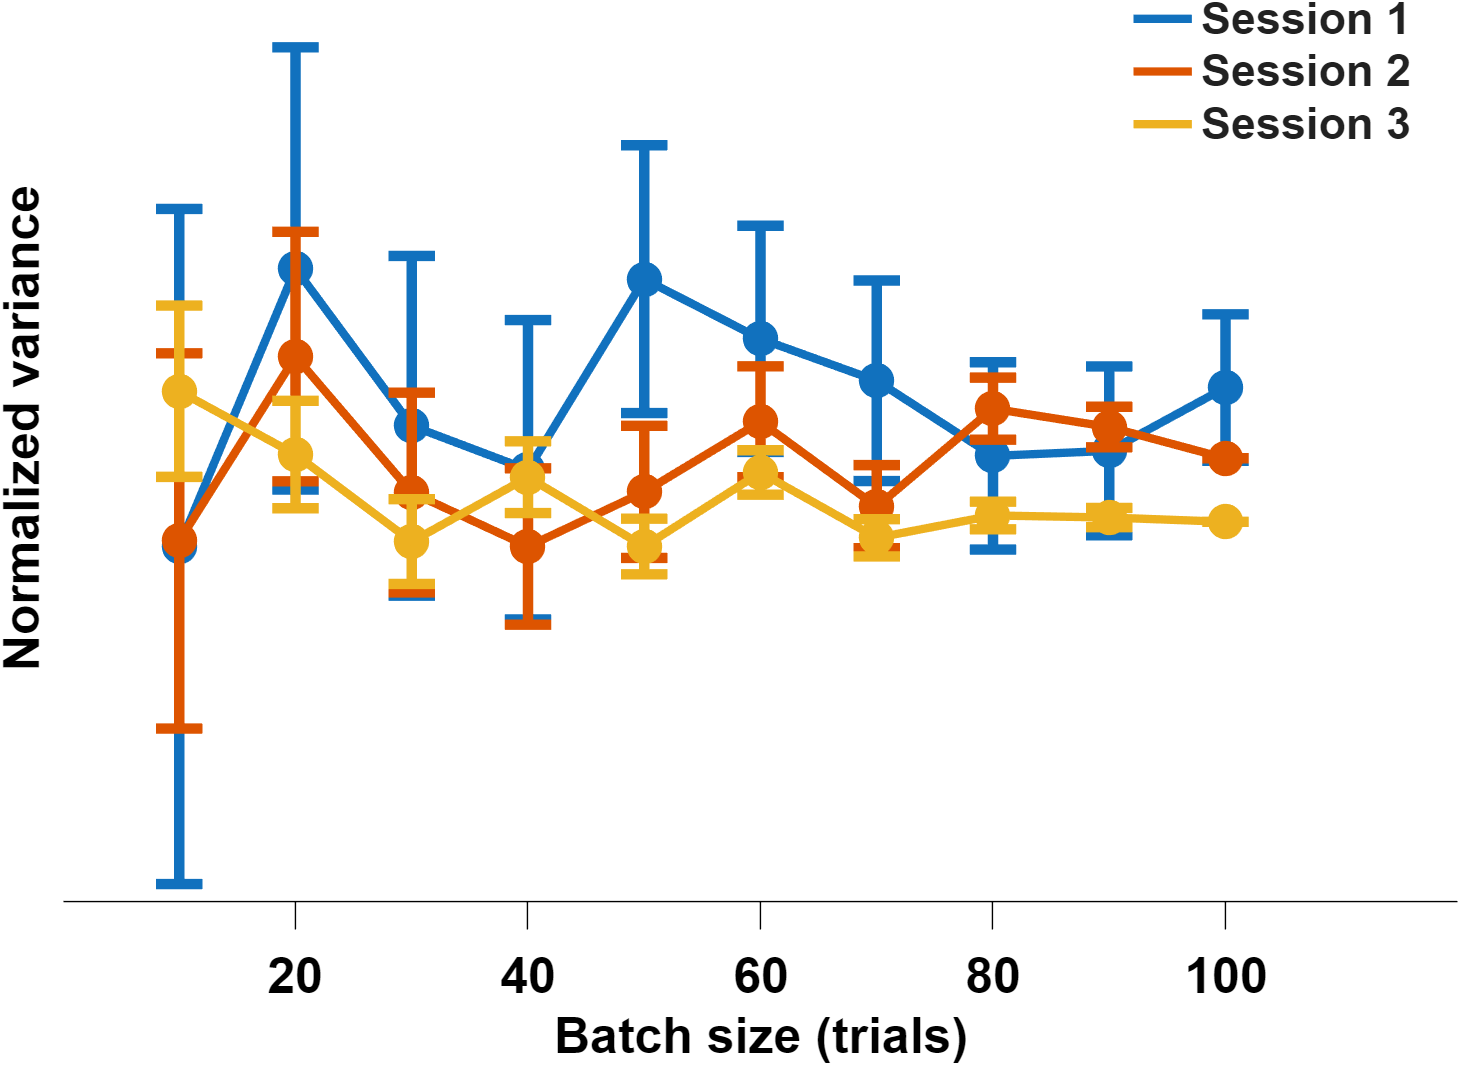
\includegraphics[width=0.5\linewidth]{images/spont_variance.png}
    \caption{Convergence of trial-averaged $\Delta F/F$ variance with batch size, supporting the trial-averaging assumption. Mean total variance $\mathrm{Var}(y_t)$, averaged across the spontaneous-activity window and over five independent random subsamples per batch size, plotted as a function of the number of trials $N$ included in the average. Each line is one session. Variance stabilizes beyond approximately 50 trials per session, indicating that the 100-trial validation blocks provide a reliable estimate of the trial-averaged response.}
    \label{fig:S1}
\end{figure}